% Chapter 3

\chapter{ Related work }
\label{Chapter3}
\lhead{Chapter 3. \emph{ Related work }}

\section{Über- and micro-shaders}

A popular approach at tackling the shader permutation problem is the \emph{ über-shader }. In this technique, the programmer creates a huge monolithic shader containing all the features a rendered object might need. Subsets of the functionality are then selected either at compile-time via preprocessor-based conditional compilation or at run-time via dynamic branching.

TODO: example

While conceptually simple and easy to implement, the über-shader approach is hard to debug and maintain. A more advanced take at the problem is to keep shader fragments separate and merge them conditionally using run-time logic or conservatively, yet statically generate permutations in the content pipeline. \citet{Hargreaves04} shows an approach based on runtime shader fragment combining. His implementation relies on a simple extension of the HLSL language in order to define the \emph{imports} and \emph{exports} of a shader fragment. Along with a special \emph{interface block}, a preprocessor is able to combine shader fragments together, linking their inputs and outputs. This effectively hides the complexity from the shader author, making maintenance and debugging easier. Hargreaves praises the robustness of this solution and mentions that it allows the usage of the same shader fragments in various rendering algorithms.

This work builds on shader fragment merging and extends it with automatic parameter type coercion and functional composition. I show how to implement such a scheme in a way that's easy to work with even for non-programmers.

% http://books.google.com/books?id=DgMSb_10l7IC&pg=PA555&lpg=PA555&dq=%22uber+shaders%22&source=bl&ots=-mu34jRtzO&sig=C3KIgqPIb6F8MDsOU0tSevVuN8M&hl=en&ei=zPZpTNGHNoGA4Aam1aHJCQ&sa=X&oi=book_result&ct=result&resnum=4&ved=0CCIQ6AEwAzgK#v=onepage&q=%22uber%20shaders%22&f=false

\section{RenderMan}

% TODO: Keyframe: NB PRMan is now called only Renderman, not PRMan (PhotoRealistic Renderman) anymore
% TODO: the name is also a pun on Point Reyes

When designing a graphics rendering system, it's impossible not to bump into what's currently the industry standard for film rendering - RenderMan. Despite being over 20 years old, it continues to thrive as the benchmark for all rendering technology. It has been used in several dozen successful feature film productions and among its awards is the first Oscar even awarded to the developers of a software package \cite{RenderManAwards}. An interesting aspect concerning RenderMan is that the overall structure of its Interface Specification (\emph{RISpec} in short) has survived mostly unchanged since its first publication in 1988.

The rendering algorithm mainly utilized by Pixar's flagship implementation of RenderMan is called \textbf{REYES} (acronym for \emph{Renders Everything You Ever Saw}). It can be divided into the following steps:
	
\begin{enumerate}
\item \textbf{Bound} --- Conservatively cull off-screen objects using their bounding volumes. This early-out mechanism allows many calculations to be skipped for objects which can be trivially shown not to contribute to the final image.
\item \textbf{Split} --- Perform primitive-specific subdivision of the incoming geometry, generating more primitives as a result. Steps 1 -- 2 are evaluated recursively until the size of primitives meets a pre-specified threshold or a primitive declares that it's not splittable.
\item \textbf{Dice} --- Create a grid of micropolygons from each primitive generated by the previous step. Each micropolygon is a quadrilateral approximately $^1/_2$ pixel on a side. Micropolygons can be generated in a pattern matching the orientation of a texture applied to the primitive, enhancing quality via simplified filtering and improving performance due to access locality.
\item \textbf{Shade} --- Compute the lighting and shading at each vertex of the micropolygon grid.
\item \textbf{Sample} --- Generate the final image by stochastically sampling micropolygons for each pixel.
\end{enumerate}

It may seem that the algorithm is overly complex, especially when compared with regular rasterization, however it is able to exploit texture and geometric locality, parallelism and scales gracefully with increased scene complexity (\cite{Cook87reyes}). Stochastic sampling of micropolygons enables efficient computation of motion blur and depth of field effects. Finally, arbitrary primitive types can be used, as long as they can be split or diced and finally converted into micropolygons.

The architecture is programmable via 5 \emph{shader} types (\cite{keyframeRSL1}):

\begin{description}
\item[Surface] --- Defines how a surface reacts to light, allowing the programmer to define its look. Surface shaders allow custom reflectance models to be defined, but also specify how the pigment or material of an object looks, hence allowing the definition of complete \emph{BRDF}s.
\item[Displacement] --- These shaders change the macro-structure of the surface, being able to change normal vectors or offset the positions of micropolygons.
\item[Volume] --- Changes the color of light rays as they travel through a volume. May be used to create effects such as fog or smoke.
\item[Light] --- Represents the light source, allowing specification of light colors, shadows, intensity, falloff, barn doors, etc. Computes the amount of lights which arrives at a particular point in space -- the surface being shaded.
\item[Imager] --- Imager shaders operate on the image pixels just prior to the final output. They may be used e.g. to perform color correction or procedural background generation. Unfortunately, an imager shader being run for a single output pixel may only use the corresponding single pixel as an input, so more advanced effects, such as tone mapping are not feasible.
\end{description}

An important aspect of the RenderMan architecture is its ability to freely mix and match any primitives and shaders. Since every primitive eventually resolves to micropolygons, it can be used with any \emph{Displacement}, then processed by any \emph{Surface} shader. The latter may in turn interact with any \emph{Light} shaders, hence ensuring full orthogonality of the building blocks.

Unfortunately, micropolygon-based real-time rendering is still not viable for current commodity hardware. Nevertheless, there have been numerous attempts at an implementation. TODO: refs (render ants, a lot from Siggraph 2010). A prominent issue exists with the current GPUs not scaling well to sub-pixel-sized polygons, resulting in up to 8 times more shading work than what would seem to be required (TODO: ref).

Still, even without using micropolygon-based rendering, an architecture can be developed which retains some of the advantages RenderMan possesses. In particular, this thesis presents a shading framework decoupled from the domains imposed by current GPUs, instead being closer to the model employed by RenderMan. Additionally, the limitation of \emph{Imager} shaders is lifted, hence enabling more sophisticated post-processing effects to be created.

\section{Deferred rendering}

The standard \emph{Forward} rasterization algorithm requires that material and light shaders for an objects be merged into a single GPU program. The implications are two-fold:
\begin{enumerate}
\item The lower bound on the number of GPU programs that need to be compiled is $O(m * l)$ (where $m$ stands for the number of materials and $l$ for the number of light shader \emph{combinations}), or \emph{multi-pass} rendering must be used.

As explained in chapter 2 [TODO: ref], the number of shaders created this way would be prohibitively large. A workaround is to restrict the possible light shader combinations. This may be achieved via über-lights \cite{UberLights, UberLightsCg} or just constraining the renderer to a handful of light types. Additionally, a common approach may be to fit a shader for more lights than an object is affected by by zeroing-out the non-existent light intensities. For instance, when the renderer must render an object influenced by two point-lights, it may use a shader for rendering it with three point-lights, assuming zero intensity for one of the shader parameters. Naturally, this approach, just like the über-light one, carries a runtime cost which may be prohibitive for a complex setup.

An alternative approach to this issue is \emph{multi-pass} rendering, where the object is rendered once for an affecting light, and the resulting illumination is summed via additive blending. The downside to this solution is that in scenes with complex geometry, rendering objects multiple times will quickly drain the computational budget.

\item Lights can only influence the scene at the granularity of individual objects, not their vertices or rasterized pixels. Even when a light would affect a small part of an object, it must be evaluated for all elements thereof, because a single \emph{batch} may only use a single shader per domain.

Splitting objects into smaller pieces might be an option, however GPU batch submission carries a nontrivial cost \cite{BatchBatchBatch}, hence the tendency is to do the exact opposite.
% TODO: explain shader domains
\end{enumerate}

Recently a technique known as \emph{deferred shading} has been gaining popularity, as it offers an elegant solution to both of these problems. Originally proposed in \citet{DeeringDeferred}, the algorithm separates the rendering pipeline into two stages:

\begin{enumerate}
\item Render surface attributes of the visible scene into a set of framebuffers \emph{(collectively called the \textbf{G-buffer})}.
\item For each light, evaluate its contribution on the surfaces encoded within a subset of the buffers.
\end{enumerate}

TODO: Decouples light / reflectance shaders from material shaders. Neat, but limited BRDFs, problems with transparency.

\subsection{Deferred lighting}

% TODO: ref the olde nvidia paper
The regular deferred rendering algorithm requires a large G-buffer [TODO: ref Killzone2], which in some cases may be prohibitive due to memory capacity or bandwidth constraints. \citet{Engel08PrePass} proposes an alternative approach, currently known \emph{light pre-pass}, \emph{deferred lighting} or \emph{pre-lighting}. Unlike classical deferred rendering, which consists of two phases, this algorithm is composed of three stages:

\begin{enumerate}
\item Render a minimal G-buffer, containing the surface depth and normal.
\item For each light, evaluate its contribution on the surfaces encoded within a subset of the buffers using only the reflectance model.
\item Render scene objects again, this time fully evaluating their materials and combining them with the illumination computed in the previous step.
\end{enumerate}

% http://http.developer.nvidia.com/GPUGems2/gpugems2_chapter09.html

\section{Graph-based systems}

TODO: Graph-based nice for artists, short turn-around time. Need to communicate well and not have artists go too wild [ref Christer]. Projects successfully shipped with this approach, more being created, but must still have a way to go down into code and do stuff intuitively, otherwise it's just moving the programming into retarded graphs.

\subsection{Frostbite}

TODO: Uses surface shaders, not much info about the other kinds which Renderman provides. Not going away for Frostbite2, a few titles shipped, so probably works out just fine.

\subsection{Mental Mill}

TODO: Seems nice on paper, however custom access to lights from MetaSL looks problematic from the point of view of automatically adapting its shaders to various algorithms.

\subsection{Abstract Shade Trees}

\citet{mcguire2006shadetrees} introduce \emph{Abstract Shade Trees} which offer an interesting solution to the type mismatch problem mentioned byAbram and Whitted. The key concept in their approach is embedding \emph{semantic} information in types used to define the interfaces of computational atoms. This enables a \emph{weaver} algorithm to automatically connect the atoms and perform type coercions.

They note that regular types used by a shading language such as GLSL are "merely C-style storage specifiers with little value as abstractions. For example, a color, a 3D location, and a row of a 3×3 matrix have the same type, which is also indistinguishable from an array of three floating-point numbers." Their \emph{semantic types} are able to carry more meaningful information, such as:
\begin{itemize}
\item The \textbf{Basis} in which instances of this type are defined (tangent, object, world, screen).
\item \textbf{Length} of a vector (unit, any).
\item The very interpretation, e.g. whether it’s a color, a texture coordinate or a normal vector.
\end{itemize}

Such a type system allows stronger checking, but it also enables automating tedious tasks such as coordinate-space conversions. For example, when one atom outputs a position vector in \emph{object} space, and another requires the position in \emph{world} space, it's possible to generate code to perform the required math.

\begin{figure}[h!]
  \centering
    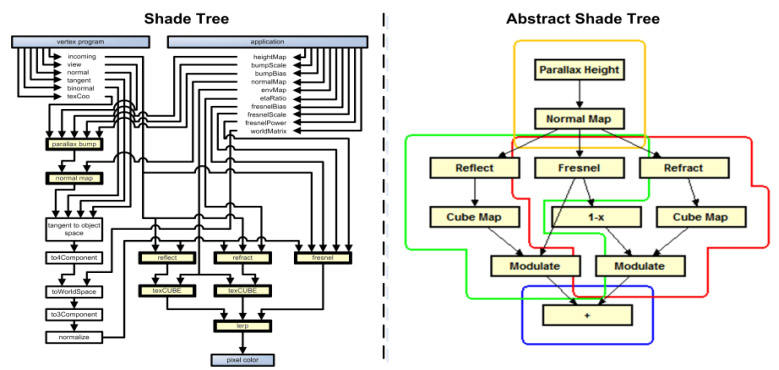
\includegraphics[width=0.9\linewidth]{./Chapters/AbstractShadeTree.jpg}
    \caption[Abstract Shade Tree]{A conventional Shade Tree (left) and the equivalent Abstract Shade Tree (right). Image courtesy of McGuire et al.}
  \label{fig:AbstractShadeTree}
\end{figure}

An \emph{Abstract Shade Tree} is normally much more compact than an equivalent \emph{conventional Shade Tree}, as demonstrated by Figure \ref{fig:AbstractShadeTree}. Thanks to the complexity hiding, shader authoring becomes less error prone and especially easier for users who do not have knowledge of programming concepts such as types, variables or the vector math used to implement algorithms inside the atoms.
 
% TODO: cite Abram and Whitted's work in the beginning of the section

The rendering system presented in this work utilizes a \emph{semantic type system}, however it's not central to its function. Manual connections of inputs and outputs are allowed in addition to setting coarse-grained dependencies between atoms. Both the former and the latter are then subject to automatic type coercions, hence type safety is retained. I also extend the work of McGuire et al. with the introduction of \emph{semantic expressions}, which provide parametric polymorphism and basic type algebra for atom parameters.

\section{Permutation management}

TODO: Unity3D and Frostbite - Statically generate lots of shaders.

TODO: Tri-Ace - Storing of shader permutations generated via play-testing instead of static generation of many combinations.
